%% ---------------------------------------------------------------------------------------------------------
\section{Vision-CENTER V2}\label{sec:method}

Figure~\ref{fig:method} summarises the controller; this section describes it as implemented (constants in Supplementary Table~S2). Its design follows a development observation: in 100 diagnostic scenes, the 14 failures in which the frozen policy released the held cube over the target let go of it 1.7--4.7\,cm off-centre, whereas successful releases were at most 2.3\,cm off-centre (a post hoc reading; Supplementary Section~S2). A privileged centring move at the release instant then turned 10 failures into successes without harm on 100 further development scenes, so the remaining problem was to estimate the offset from observations alone.

\begin{figure}[!htbp]
\centering
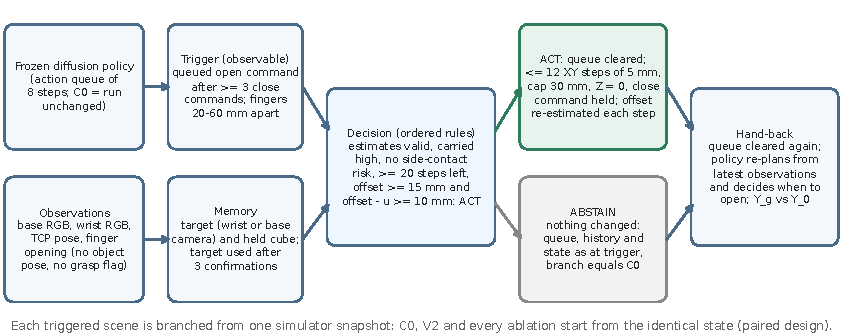
\includegraphics[width=\linewidth]{Fig02_method.pdf}
\caption{Vision-CENTER V2 as implemented. The trigger is an observable rule on the policy's own commands and the finger opening. At the trigger the controller combines current base- and wrist-camera estimates with a confirmed target memory and a held-cube memory. If it abstains, nothing is changed and the branch equals C0. If it acts, the policy's action queue is cleared, horizontal steps of at most 5\,mm are commanded with zero vertical command and the held close command, the offset is re-estimated after every step, and at the end the queue is cleared again so that the frozen policy re-plans from its latest observations. Every arm is branched from the same simulator snapshot.}\label{fig:method}
\end{figure}

\paragraph{Trigger} The trigger fires at the first control step at which three observable conditions hold: the gripper component of the policy's next queued action is an open command; the policy's last three or more executed gripper commands were close commands; and the finger opening (sum of the two finger joints) is between 0.02 and 0.06\,m, i.e.\ neither empty nor fully open. The rule does not read whether, or which, object is grasped. It can therefore fire when the fingers hold the wrong object: in development scene 51152 (policy seed 2) the policy had grasped the \emph{target} cube; every vision arm, including V2, abstained there for lack of a held-cube estimate, and only the privileged oracle moved (Section~\ref{sec:physics}). At the trigger the pending action has not yet been executed. If the controller abstains, the simulator state, the action queue, the observation history and the counters are left untouched (checked in every run), so the branch is identical to C0.

\paragraph{Observations} The controller receives the base and wrist RGB images ($128\times128$ each), the TCP pose, the finger opening and the last executed gripper command. Cubes are located by colour segmentation and projected with the fixed camera parameters; no model is trained.

\paragraph{Memory} The target cube is often hidden by the held cube at the trigger, so V2 keeps two memories, updated at every step from the start of the episode. The \emph{target memory} stores one position with a reading bound $u$: a step with an accepted wrist-camera fit ($u=2$\,mm) updates it, otherwise a step with an accepted base-camera estimate ($u=5$\,mm) does. An observation consistent with the stored position (distance at most the sum of the two bounds) increases its confirmation count, and the more precise source keeps the position; an inconsistent one replaces it and restarts the count. The memory is used only after $m=3$ confirmations, its bound grows by 5\,mm if the gripper passed close to it unobserved, and it is refused if the current image contradicts it. Its source is recorded as \emph{hand} or \emph{base} memory. The \emph{hold memory} stores the held cube's position relative to the gripper; it is refitted every fourth step while the gripper is commanded closed ($u=2$\,mm) and dropped when the finger opening changes by more than 1\,mm. At the trigger, an accepted estimate from the current frame is preferred, otherwise the memory is used.

\paragraph{Decision} Let $\hat{\mathbf{o}}=\hat{\mathbf{x}}_{\mathrm{target}}-\hat{\mathbf{x}}_{\mathrm{held}}$ be the estimated horizontal offset and $u$ the bound of the target estimate. The rules are evaluated in a fixed order and the first that applies decides: no held-cube estimate, no target estimate, or memory contradicted (abstain); held cube centre estimated below 58\,mm, or a remembered target with the held cube's bottom below the target's top face (\textsc{low carry}); offset at least 40\,mm (plus $u$ for a remembered target) with less than 3\,mm vertical clearance (\textsc{side-contact risk}); fewer than 20 steps left in the episode; $\|\hat{\mathbf{o}}\|<15$\,mm (\textsc{aligned}); $\|\hat{\mathbf{o}}\|-u<10$\,mm (\textsc{aligned within uncertainty}). Otherwise V2 acts, so acting requires
\begin{equation}
\|\hat{\mathbf{o}}\| \;\ge\; 15\ \mathrm{mm} \qquad\text{and}\qquad \|\hat{\mathbf{o}}\| - u \;\ge\; 10\ \mathrm{mm}.
\end{equation}

\paragraph{Bounded move} If V2 acts, it clears the policy's action queue (the pending open command is discarded) and, at each control step $t$, commands a horizontal TCP increment $\Delta\mathbf{x}_t$ towards the current offset estimate with
\begin{equation}
\|\Delta\mathbf{x}_t\|\le 5\ \mathrm{mm},\qquad \|\mathbf{x}_t+\Delta\mathbf{x}_t-\mathbf{x}_{t^\star}\|\le 30\ \mathrm{mm},\qquad t-t^\star< 12,
\end{equation}
where $\mathbf{x}_t$ is the measured TCP position and $\mathbf{x}_{t^\star}$ the TCP position at the trigger. The action sent to the end-effector delta-position controller has zero vertical component and repeats the last executed gripper command, which is a close command, so the grasp command is held rather than absent. No policy inference runs during the move (checked). After every step the images are read again and the offset is re-estimated, so the move is closed-loop on vision. It stops when the estimated residual is within 10\,mm (5\,mm when the target comes from memory), after 12 steps, at the target cap, at the end of the episode, or when the target estimate jumps by more than 3\,mm (plus $u$ for a remembered target), the estimate is lost, the held cube drops below 58\,mm, or the held cube shifts in the gripper by more than 3\,mm. Every step is charged to the 200-step episode budget.

\paragraph{Hand-back} At the end of the move the queue is cleared again. At the next step the frozen policy infers a new action chunk from its observation history, which now contains the observations made during the move; the policy decides when to open the gripper. In every acted V2 branch of all stages the policy re-planned at the first step after the move, and its first open command followed 1--24 steps later (median 2--3 by stage and policy); in one calibration branch it never opened the gripper again (Supplementary Table~S4).

\paragraph{Executed motion} The arm covered less than the commanded path: over all acted development branches, the net horizontal TCP displacement was 26--40\% of the commanded path length (medians 36\% and 37\% for the two policies), so 12 steps moved the TCP by roughly 20--25\,mm. This is an observed property of the controller in this simulator, not a bound. No V2 move ended at the 30\,mm cap; moves ended at the estimated tolerance or at the step budget. Offsets much larger than one move can remove are therefore only partly corrected (Section~\ref{sec:mechanism}).

\paragraph{Ablations and reference} \emph{V1} uses the wrist camera only and no memory. \emph{V2 single frame} gives V2 an empty memory until the trigger and lets it use only the trigger step's observation; because one frame cannot provide three confirmations, it accepts a single estimate ($m=1$), which favours this arm. \emph{V2 without hand / base / hold memory} prevents wrist-camera fits, base-camera estimates or held-cube fits from entering the memory. \emph{V2 rules off} keeps the full memory and removes, as one bundle, the three V2-specific rules (\textsc{aligned within uncertainty}, \textsc{side-contact risk}, and the \textsc{low carry} rule for a remembered target); the estimate-validity rules, the height rule, the step-budget rule and the 15\,mm rule inherited from V1 remain. \emph{Oracle centring} replaces the estimates by the true cube positions and is privileged.
